\chapter{Analysis of Posteriors and Inference by Enumeration}

In a model as complex as a generative scene graph program, it becomes essential to carefully check and analyze the behavior of the posterior to ensure it is a good representation of the data.
We conduct a set of synthetic experiments that carefully inspect isolated aspects of our model to ensure their posteriors exhibit reasonable behavior that conforms to intuition.

\section{Enumerative Inference}
In conducting an analysis of a generative scene graph program, we would like to inspect the posterior distribution under different scene configurations.
Calculating the full posterior is intractable (indeed, this is why we have to perform inference in the first place).
However, by conditioning the model on specific settings for most of the latent values, we can reasonably enumerate over a small set of free variables, and plot the posterior distribution over a \textit{projection} of our model to a lower dimensional slice.
We note that this approach is limited in its ability to examine interactions between variables, and in generality the posterior of the full model can exhibit very different behavior from isolated projections to lower dimensions.
Nonetheless, we show that these projections can still be a rich source of information for understanding and improving scene graph priors.

\section{Structure Posterior}
The first analysis we conduct looks at the model's predictions for structure between objects, as a function of the observed vertical offset $y$ between their closest faces.
We consider the static model and dynamic model respectively, and look at the behavior of the structure posterior under multiple settings of their hyperparameters.
We demonstrate the high variability of the qualitative behavior of the posterior under different settings for hyperparameters; this in turn shows the vital importance of proper hyperparameter tuning in ensuring the correctness of scene graph models.
\begin{figure}[h]
  \centering
  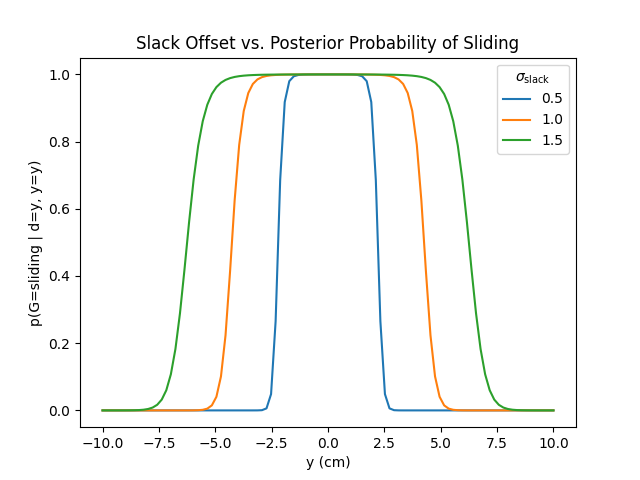
\includegraphics[width=0.9\columnwidth]{posStructurePosterior}
  \caption{
    Probability that an object is sliding in a static scene with different settings of $\sigma_\mathrm{slack}$, and observed/latent vertical offset $y$.
  }
  \label{fig:posStructurePosterior}
\end{figure}

\subsection{Static Model}
We set up an experimental scene with two objects, to visualize the enumerated structure posterior for $G$.
given an observed vertical offset $y$ between the object's closest faces.
We restrict our latent parameters to be the same as the observed poses, and for the two observed poses to be the same, except for a one-dimensional vertical offset $y$ between their closest faces.
We set the structure prior to be uniform, so all structures have equal prior probability.
Recall the slack offset model is a normal distribution with standard deviation $\sigma_\mathrm{slack}$.

Figure~\ref{posStructurePosterior} shows the posterior probability that $G$ is a ``sliding'' configuration, given an offset $y$, for a few different settings of $\sigma_\mathrm{slack}$.
Predictably, the wider the distribution on slack, the larger a gap the model is willing to allow while still classifying the objects as ``sliding''.
We also note the relatively sharp transition in the sliding probability from almost 0 to almost 1, at a discrete cutoff point; as we will examine later this could be a result of a poor model for our slack variable.

\subsection{Dynamic Model}
\begin{figure}[H]
  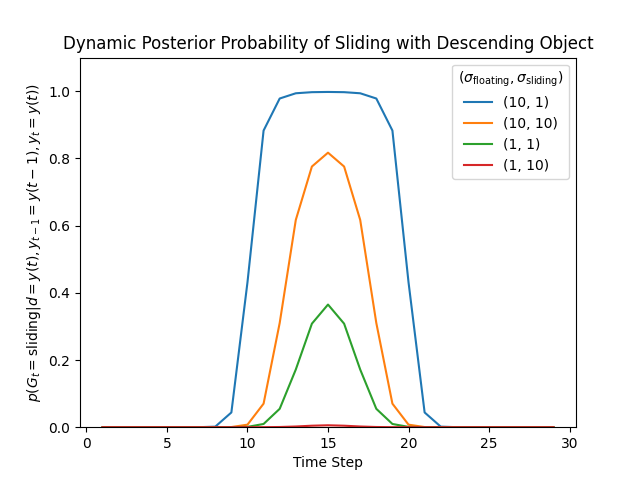
\includegraphics[width=\columnwidth]{dynamicStructurePosterior}
  \caption{
    Probability that the scene structure $G_t$ is in a ``sliding'' configuration at time $t$, in a dynamic scene where the object's observed position and slack offset is given by $y(t) = 10 - 0.67\cdot t$ cm, with hyperparameters $(\sigma_\mathrm{floating}, \sigma_\mathrm{sliding})$.
  }
  \label{fig:dynamicStructurePosterior}
\end{figure}
The second experimental scene is very similar to the first, except we introduce a dynamic element to examine the effect of the dynamics parameters.
Across 30 time steps, the top object (and its observation) is lowered along the vertical offset from 10 cm above the bottom object, to 10 cm interpenetrating with the bottom object.
For simplicity, we again set the prior structure at each time step to be uniform and temporally independent.
We set $\sigma_\mathrm{slack} = 1 cm$, and recall that the floating position dynamics are a 3D normal distribution with standard deviation $\sigma_\mathrm{floating}$, while the sliding dynamics are a 2D normal distribution with standard deviation $\sigma_\mathrm{sliding}$.

Figure~\ref{fig:dynamicStructurePosterior} shows the posterior probability that $G_t$ is a ``sliding'' configuration, given the observed/latent offset $y$, for each time step $t$ of the dynamic scene.
Adding dynamics has added completely new behavior to the structure posterior, dependent on the additional hyperparameters.
The pose displacement is always $2/3$ cm every time step, meaning the most accurate dynamics model in this figure is the one with the tightest distribution.
The change in posterior probability in sliding structure is a consequence of the Bayesian Occam's Razor; the posterior probability for sliding is greatest (blue curve) when the sliding dynamics model is much more confident (concentrated) than the floating dynamics model, and is least in the opposite case (red curve).
This is our first encounter with the Bayesian Occam's Razor adding complications to the development of scene graph models, but as we shall see there are several cases where the concentration of our different models have a huge impact on the behavior of the posterior.

\begin{figure}[H]
  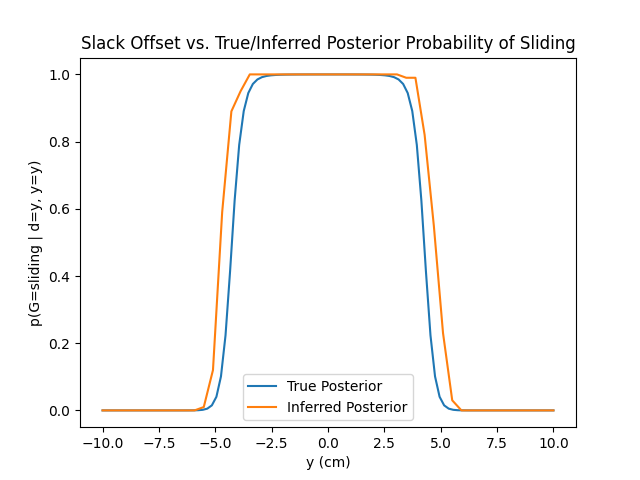
\includegraphics[width=\columnwidth]{inferredStructurePosterior}
  \caption{
    RJMCMC structure inference results.
    For each value of $d$, we infer the approximate probability of sliding as the average structure of 100 particles run with 3 iterations of our RJMCMC algorithm applied to the top object.
  }
  \label{fig:inferredStructurePosterior}
\end{figure}

\subsection{RJMCMC Structure Inference}
Finally, we include a brief comparison of our RJMCMC inference procedure to the enumerated posterior.
We replicate the scenario shown in Figure~\ref{fig:posStructurePosterior} with $\sigma_\mathrm{slack} = 1$ cm, and overlay the inferred posterior probability of a sliding structure.
As we can see, RJMCMC accurately recovers the posterior in this situation, which is a successful first test of the correctness of our algorithmic implementation.

\section{Contact Slack Model}
The second analysis we conduct examines the enumerated posterior over the model for slack offset $d$.
Having a good slack model is important for having a good structure model; if the slack model provides a poor explanation for any observed gap between ``contacting'' objects, the structured model will also provide a poor explanation for the scene.
Recall our prior model over slack is $p_\mathrm{norm(0,\sigma_\mathrm{slack})}(d)$.

\begin{figure}[h]
  \centering
  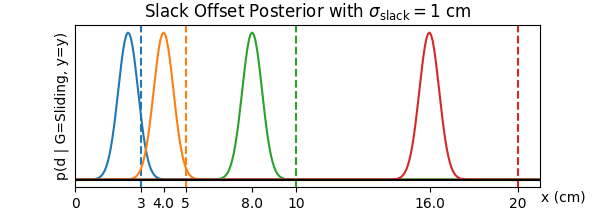
\includegraphics[width=\columnwidth]{slackOffsetPosterior}
  \caption{
    Posterior distribution on slack offset $d$.
    The dashed lines represent the set of observed $y$ values, while the curve of the same color represents the slack offset posterior, given the observed $y$ and sliding structure.
  }
  \label{fig:slackOffsetPosterior}
\end{figure}

\subsection{Varying the Gap between Sliding Objects}
We set up an experimental scene with two objects, to visualize the enumerated slack offset posterior for $d$, given a fixed sliding structure.
We restrict our objects to share the same observed pose, except for a one-dimensional vertical offset $y$ between their contacting faces.
In our prior model we set $\sigma_\mathrm{slack} = 1$ cm and $\sigma_\mathrm{inlier} = 0.5$ cm.
Figure~\ref{fig:slackOffsetPosterior} shows the posteriors corresponding to various settings of the observed offset $y$.
Because our $p(d | G=\mathrm{sliding}, y=y) = p_\mathrm{obs}(d | y=y) \cdot p_\mathrm{slack}(d)$ is a product of normal distributions, the posterior is also a normal distribution with mean in-between the mean of the two model distributions.
This means the most probable gap between two objects given a sliding structure is counter-intuitively in-between 0 and the observed gap $y$; this may explain why we see such sharp cutoffs in the probability of a sliding structure in Figures~\ref{fig:posStructurePosterior} and \ref{fig:dynamicStructurePosterior}.
As the observed gap between two objects becomes larger, the model over slack offset quickly becomes a poor explanation of the observation.
A more reasonable model would place high mass around $d = y$, as this would explain the observation most accurately.

\subsection{Hyperprior over Slack Standard Deviation}
To improve the model, we consider adding a hyperprior over $\sigma_\mathrm{slack}$, to more accurately allow for uncertainty in the size of the slack term.
We introduce an exponential distribution with rate parameter $\lambda = 0.2$ over the slack standard deviation $\sigma_\mathrm{slack} \sample \mathrm{Exp}(0.2)$.
Figure~\ref{fig:jointSlackHyperpriorPosterior} shows the joint posterior over $\sigma_\mathrm{slack}$ and the slack offset $d$.
The figure shows that the mode of the posterior is located much closer to the observation than without a hyperprior over $\sigma_\mathrm{slack}$.
Indeed, as we see in Figure~\ref{fig:jointSlackHyperpriorPosterior}, the posterior exhibits much more reasonable behavior when letting $\sigma_\mathrm{slack} = \sigma_\mathrm{slack}^*$.
We conclude that adding a hyperprior over slack is a viable way to increase the accuracy of the model with a sliding structure, especially when the observed gap between objects is large.

\begin{figure}[H]
  \centering
  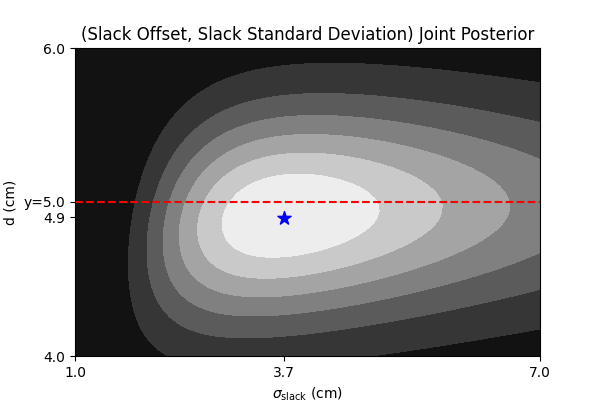
\includegraphics[width=\columnwidth]{jointSlackHyperpriorPosterior}
  \caption{
    Joint posterior $p(d,\sigma_\mathrm{slack} | y = 5.0)$.
    The dashed red line indicates the observed position $y = 5.0$ of the top object.
    The blue star indicates the maximum a posteriori $(\sigma_\mathrm{slack}^*, d^*)$.
  }
  \label{fig:jointSlackHyperpriorPosterior}
\end{figure}

\begin{figure}[H]
  \centering
  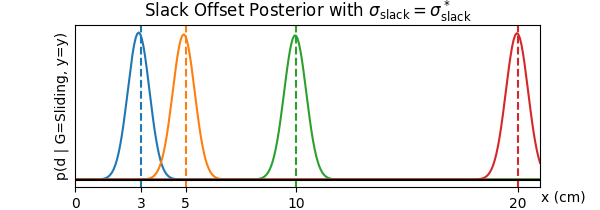
\includegraphics[width=\columnwidth]{slackOffsetPosteriorMapStdev}
  \caption{
    Slack offset posterior for $d$, conditioned on $\sigma_\mathrm{slack} = \sigma_\mathrm{slack}^*$.
    The dashed lines represent the set of observed $y$ values, while the curve of the same color represents the posterior over slack given the observed $y$ and sliding structure.
  }
  \label{fig:slackOffsetPosteriorMapStdev}
\end{figure}

\pagebreak

\section{Neural Outlier Model}
A big part of our model is leveraging a bottom-up feature detector like a neural network to leverage
A simple form of intuitive physical reasoning we model is by discouraging large changes in distance over a single time step via our normally-distributed dynamics model.
Our prior observational model is a simple mixture of a uniform outlier distribution over poses in a finite bounded box region, with component $p(\mathrm{outlier}) = 0.1$, and a direct product of a normal and VMF inlier distribution, with component $p(\mathrm{inlier}) = 0.9$.
Ideally, the product of this model and our dynamics model would allow our scene graph model to confidently predict that large leaps in our latent position over a single time step are less probable than that specific observation being an outlier ``flicker'' detection, sampled randomly within the scene.

Figure~\ref{fig:outlierModel} shows a scene in which an object's observed pose jumps from a latent position at the origin, $x_1 = 0$, to one located a distance $y_2$.
On the left, when the dynamics and observational model are equivalent width, the posterior predicts that the detection is more likely to be an outlier than not at around $y_2 = 9.6$.
On the right, when the dynamics is significantly more broad than the observational model, the posterior predicts that the detection is more likely to be an inlier, all the way up to $5 \cdot \sigma_\mathrm{floating} = 50$ cm away from the previous position.
The prior probability that an object travels a distance than $5 \cdot \sigma_\mathrm{floating}$ away from the mean is less than $5.73e-7$, which is dramatically less than the prior probability of an object being an outlier $p(\mathrm{outlier}) = 0.1$.


The model on the right is counter-intuitively claiming that the object made an extraordinarily unlikely jump.
If we examine the log probability density functions evaluated at the modes of the latent pose joint distributions, for the inlier and outlier models respectively, we begin to see why:
\begin{align*}
  \log p(x_2 = 50, y_2 = 50, \mathrm{inlier} | x_1 = 0) &= \\
  \log p(\mathrm{inlier}) &+ \\
  \log p(x_2 = 50 | x_1 = 0, \mathrm{inlier}) &+ \\
  \log p(y_2 = 50 | x_1 = 0, x_2 = 50, \mathrm{inlier}) &= \\
  -0.105 - 1.783 + 17.625 &= 15.737 \\
  \log p(x_2 = 0, y_2 = 50, \mathrm{outlier} | x_1 = 0) &= \\
  \log p(\mathrm{outlier}) &+ \\
  \log p(x_2 = 0 | x_1 = 0, \mathrm{outlier}) &+ \\
  \log p(y_2 = 50 | \mathrm{outlier}) &= \\
  -2.303 + 10.717 - (3\cdot0. + 2.289) &= 6.125
\end{align*}

The dynamics model's density weights heavily in favor of the observation being an outlier.
However, the inlier pose distribution is so tightly concentrated compared to the outlier pose model, that it dominates the calculation of the overall model weight.
The posterior tells us that the model would rather have the latent pose make an incredibly unlikely jump, if it means it can explain the observed pose confidently using the inlier observational model.
This is another occurrence of the Bayesian Occam's Razor, where the most concentrated component of the model (in this case the observation model), determines where the majority of the posterior mass is distributed.

\raggedbottom

\pagebreak

\flushbottom

\begin{figure}[H]
  \begin{subfigure}[b]{0.5\textwidth}
    \centering
    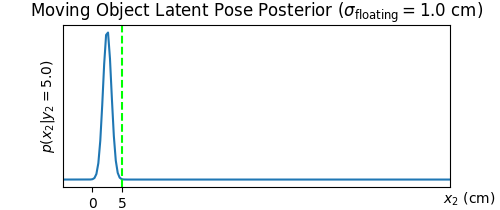
\includegraphics[width=\columnwidth]{outlierModel1a}
  \end{subfigure}%
  \begin{subfigure}[b]{0.5\textwidth}
    \centering
    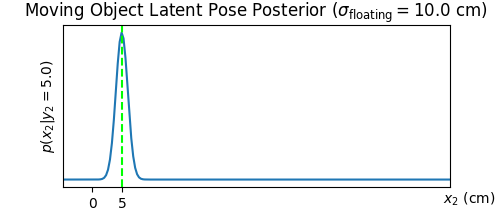
\includegraphics[width=\columnwidth]{outlierModel2a}
  \end{subfigure}
  \begin{subfigure}[b]{0.5\textwidth}
    \centering
    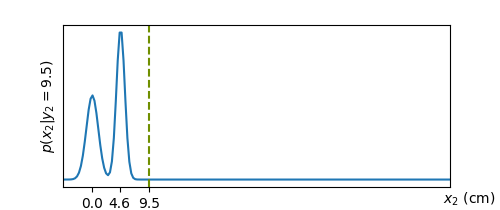
\includegraphics[width=\columnwidth]{outlierModel1b}
  \end{subfigure}%
  \begin{subfigure}[b]{0.5\textwidth}
    \centering
    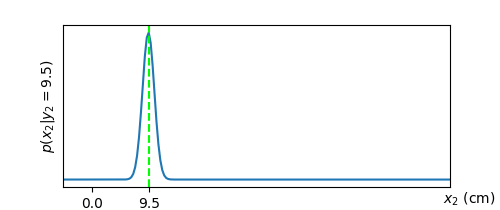
\includegraphics[width=\columnwidth]{outlierModel2b}
  \end{subfigure}
  \begin{subfigure}[b]{0.5\textwidth}
    \centering
    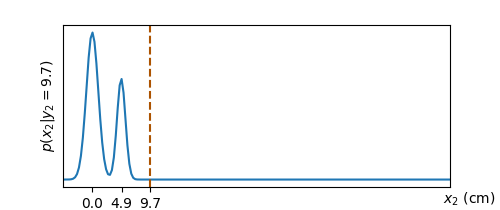
\includegraphics[width=\columnwidth]{outlierModel1c}
  \end{subfigure}%
  \begin{subfigure}[b]{0.5\textwidth}
    \centering
    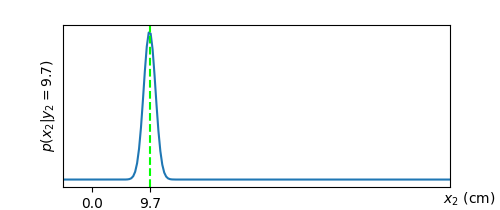
\includegraphics[width=\columnwidth]{outlierModel2c}
  \end{subfigure}
  \begin{subfigure}[b]{0.5\textwidth}
    \centering
    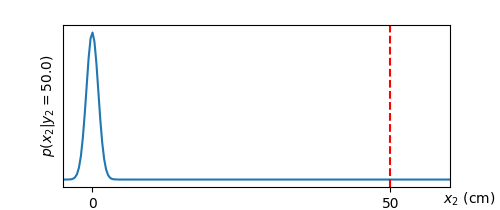
\includegraphics[width=\columnwidth]{outlierModel1d}
    \subcaption{
      Pose posteriors where $\sigma_\mathrm{floating} = \sigma_\mathrm{inlier} = 0.01$.
    }
  \end{subfigure}%
  \begin{subfigure}[b]{0.5\textwidth}
    \centering
    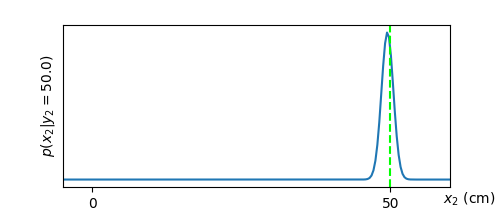
\includegraphics[width=\columnwidth]{outlierModel2d}
    \subcaption{
      Pose posteriors where $\sigma_\mathrm{floating} = 10 \cdot \sigma_\mathrm{inlier} = 0.1$.
      At all observed values for $y_2$, the model strongly classifies the detection as an inlier.
    }
  \end{subfigure}
  \caption{
    Posteriors over the latent pose of an object $p(x_2 | y_2) = p(x_2 | y_2, x_1 = 0)$, under two different settings of the dynamics parameter.
    The noisy observational model's inlier distribution is given by $\sigma_\mathrm{inlier} = 0.01$.
    The prior probability of an outlier is $0.1$.
    The dashed line represents the observed pose $y_2$, with color representing the probability that $y_2$ is an outlier (totally green means $p(\mathrm{inlier}) = 1$, while totally red means $p(\mathrm{outlier}) = 1$).
  }
  \label{fig:outlierModel}
\end{figure}

\pagebreak

\section{Lessons for Improving Scene Graph Priors}
We can take three big lessons from these experiments regarding the improvement of our scene graph model.
The first lesson is that the qualitative behavior of the posterior is highly sensitive to the proper tuning of hyperparameters.
As we saw in the structure posterior analysis, hyperparameter settings had a crucial impact on the performance of the model.
Furthermore, we saw how introducing dynamics over continuous parameters impacts the posterior probability over discrete structure.
Interactions like these can be highly counter-intuitive, and difficult to explore using synthetic tests like we've done here.
It's for this reasons that we believe in the future development of scene graph models, training model hyperparameters and analyzing model performance using real-world data will be a vital step in improving accuracy.
Next chapter we explore real-world data sets, and how they can be used to test and improve scene graph models.

The second lesson is the importance of considering how the \textit{relative} concentrations of different component distributions in the model will affect the posterior.
More specifically, the Bayesian Occam's Razor suggests that distributions with very high concentrations of their mass will tend to have an overinflated impact on where mass ends up in the posterior.
In the simplest case, the relative concentration of distributions in different model structures have a large impact on which model structures are more probable in the posterior.
In the extreme case, this can lead to entire parts of the prior model being neglected in favor of assigning high weights to areas that maximize the density of the especially peaky model component.
Uur scene graph model has a large family of possible model structures, with different continuous parameter distributions of varying concentration and dimension.
We cannot emphasize enough that \textit{all} of these distributions, and their relative concentration, matter for the calculation of the structure posterior, and thus must be considered \textit{jointly} in order to have a truly accurate understanding of the posterior in the full model.
